% Register, Not Procedure — 9pp long paper for Interpretability as a Science (NeurIPS 2026 workshop)
% Build: tectonic register_not_procedure.tex   (runs bibtex passes automatically)
%
% PROVENANCE RULE: every number in this file must trace to a row in ../numbers.md and thence to a
% committed JSON. Cells still awaiting an artifact carry a "TODO(...)" comment naming the run that
% produces them. Do not fill a TODO from memory.
%
% TODO(template): the venue's 2026 template was not yet published when this skeleton was built;
% neurips_2023.sty is a placeholder. Swap the \usepackage line when the real template lands.
% Submission mode (no [final]) keeps the author block anonymous.

\documentclass{article}

\usepackage{neurips_2023}

\usepackage[utf8]{inputenc}
\usepackage[T1]{fontenc}
\usepackage{hyperref}
\usepackage{url}
\usepackage{booktabs}
\usepackage{amsmath}
\usepackage{amssymb}
\usepackage{microtype}
\usepackage{graphicx}
\usepackage{enumitem}
\usepackage{caption}
\usepackage{multirow}

\setlist[itemize]{nosep,leftmargin=1.4em,topsep=2pt}
\captionsetup{skip=4pt}

\newcommand{\ci}[2]{{[#1,\,#2]}}

\title{Register, Not Procedure: What a Conditional Linear Map\\Can and Cannot Install}

\author{%
  Anonymous Author(s)
}

\begin{document}

\maketitle

\begin{abstract}
Activation steering and parameter-efficient finetuning both edit a model's behavior, and both can be
written as an \emph{input-conditional affine map} of the residual stream, $h \mapsto h + (Wh+b)$.
We hold this one map family fixed and sweep the \emph{task}, asking a single question under one
protocol: does the capability install? The boundary is sharp and reproducible. The map installs and
transports a \textbf{register} --- refusal tone, an answer format --- reaching the harmful-refusal
axis where every fixed-vector baseline stays at zero, and installing a commonsense donor's response
format essentially completely ($0.97$ at one layer against a $0.004$ base). Yet the identical
machinery recovers ${\approx}0$ of a reasoning LoRA's gain on either multi-step \textbf{procedure}
we test --- GSM8K arithmetic and open-book multi-hop QA --- as do MLP, on-policy DAgger,
per-context, and task-loss (DAS) variants. The null is narrower than it first appears and we state
it in the form the evidence supports: \emph{a procedure does not transport through a fitted
pointwise map at a single layer}. Concurrent work reaches finetuning-level reasoning with adapters
trained on the task and applied at every block; our mechanism analysis says why that is the shape
the problem requires: the procedure is a distributed, time-dense trajectory state (recovery needs
${\geq}94\%$ of decode steps and ${\sim}80\%$ of the residual's variance band), not a pointwise
function of the activation. Running the full battery on a register task closes the loop from the
other side: the register's full-state oracle has an earlier, sharper onset than either procedure's,
its map transports the format but \emph{destroys the answer selection the base already had}, and no
vector estimated once --- per-problem or pooled --- installs anything at all. Every null is anchored
to a positive control on the same instrument, so a null here means \emph{not installable this way},
not \emph{we did not try hard enough}. All results are on the Llama-2-7B family; we state this
limitation, and the register/procedure criterion we propose, precisely enough to be falsified.
\end{abstract}

% ===================================================================================
\section{Introduction: ``is X steerable'' is not one question}
\label{sec:intro}

The steering literature asks whether a behavior can be installed by editing activations, and tends
to treat the answer as a property of the \emph{method} --- a better vector, a learned gate, a
higher-rank edit. This paper argues the answer is dominated by a property of the \emph{behavior}.
We fix a single instrument --- a closed-form, input-conditional affine map of the residual stream,
the same object that parameter-efficient finetuning learns --- and point it, unchanged, at behaviors
of two kinds. A \textbf{register} is a disposition legible at each position: a refusal tone, a
response format, an answer template. A \textbf{procedure} is a multi-step trajectory whose steps
consume what earlier steps produced: chain-of-thought arithmetic, multi-hop composition.

Held to one protocol, the two kinds separate on every axis we measure, and the separation survives
its own controls. The map installs registers (\S\ref{sec:refusal}, \S\ref{sec:battery}) and never
installs procedures (\S\ref{sec:ladder}, \S\ref{sec:multihop}); the full-state oracle that anchors
every null recovers procedures only when it is distributed and temporally dense
(\S\ref{sec:mechanism}), and recovers a register earlier, more sharply, and more completely
(\S\ref{sec:battery}); and where the map \emph{does} leak on a procedure, the leaked component
turns out to be the task-agnostic register push, not the procedure (\S\ref{sec:multihop}).

At a venue whose stated topics are measurement validity and falsifiability, the design commitment
matters as much as the findings. Every null in this paper is anchored to a positive control on the
same driver and scored on the same contrast set, so a zero is evidence about the behavior, not
about our effort. Where our own controls destroyed a claim, the retraction is reported in line
(\S\ref{sec:battery}), because the boundary we propose is only useful if it is stated in a form
that can lose.

Contributions: (i)~a two-sided, positive-controlled measurement of the register/procedure boundary
on one instrument (\S\S\ref{sec:refusal}--\ref{sec:battery}); (ii)~a mechanism account of the
procedure side --- distributed, time-dense, variance-dense --- that predicts which interventions
can work and matches concurrent results that do (\S\ref{sec:mechanism}, \S\ref{sec:related});
(iii)~a register battery showing the boundary is visible in the \emph{oracle} itself, not only in
the map, and that register installation by weight-route edits costs selection the base already had
(\S\ref{sec:battery}); (iv)~a measured criterion table for ``installability'' with every cell
sourced or marked unmeasured (\S\ref{sec:criterion}).

% ===================================================================================
\section{Related work}
\label{sec:related}

\paragraph{Steering by a fixed direction.}
The dominant paradigm adds a single vector to the residual stream. CAA \citep{rimsky2024caa} takes
the mean activation difference over contrastive pairs; ActAdd \citep{turner2023actadd} obtains a
direction from a pair of natural-language prompts; ITI \citep{li2023iti} shifts along learned
directions at selected attention heads; RepE \citep{zou2023repe} reads and controls
population-level directions for high-level concepts. For refusal specifically,
\citet{arditi2024refusal} show a \emph{one-dimensional} subspace mediates the behaviour across
thirteen chat models. These methods share a commitment we make explicit and then test: the
intervention is a \textbf{fixed offset}, identical for every input. \S\ref{sec:refusal} measures
this family against a conditional map on the same prompts and grids, and \S\ref{sec:battery}
measures it on a second register with the vector estimated per-problem and pooled.

\paragraph{Conditional and matrix-valued steering.}
The fixed-offset assumption has been relaxed several ways, and the resulting family --- an
input-dependent affine edit of the residual stream --- is occupied ground rather than something we
introduce. CAST \citep{lee2025cast} gates a CAA vector with an explicit logistic classifier, making
conditionality a bolted-on component. Conceptors \citep{postmus2024conceptors} replace the vector
with a \emph{matrix}: the steered activation is $h' = \beta_c C h$, so the shift genuinely depends
on the input, and $C = R(R + \alpha^{-2}I)^{-1}$ with $R = X^\top X/n$ is obtained in closed form.
CLAS \citep{hsu2026clas} learns an input-dependent \emph{coefficient}, $h \mapsto h + (c\cdot[h\
1])\,d$, fit by gradient descent on next-token loss. ACE \citep{marshall2024ace} decomposes
activations affinely, shows prior steering methods are subsets of terms of that decomposition, and
controls refusal across ten models up to 70B. INNSteer \citep{nguyen2026innsteer} goes further,
learning invertible nonlinear transforms that induce input-dependent updates.

Two distinctions matter for what follows. CLAS is \textbf{rank-one conditional} --- the direction
$d$ is fixed and only its magnitude adapts --- where the map we study is full-rank, so its output
direction varies with the input. Conceptors are matrix-valued and closed-form like ours, but differ
in \emph{target}: they take the second moment of a \textbf{single} activation set, yielding a
shrinkage projection onto that set's ellipsoid with no regression target, whereas we use the
\textbf{cross moment} $X^\top\delta$ of \textbf{paired} base and donor activations. That difference
--- supervision by a second model --- is the only respect in which our instrument is unusual, and we
treat it as an instrument rather than a contribution.

The register half of our result should therefore be read as consistent with this literature rather
than as competing with it. ACE in particular reports the failure mode we also observe, that purely
directional interventions produce incoherent output where affine ones do not, on far more models
than we test. Our \S\ref{sec:refusal} exists as a \textbf{positive control}: it establishes that
the apparatus we then point at procedures does install and transport a disposition.

\paragraph{Parameter-efficient finetuning as an activation edit.}
LoRA \citep{hu2022lora} learns a low-rank weight delta; LoReFT \citep{wu2024reft} learns an edit
$h + (Wh + b - hR)R^\top$ applied to hidden representations of a frozen base. The latter is,
formally, the same object as a conditional affine steering map, and the correspondence between the
two spaces is not ours to claim: \citet{adila2026weightshifts} establish a first-order equivalence
between activation-space interventions and weight-space updates, derive the conditions under which
steering can replicate finetuning, and identify the post-block output as the expressive
intervention site. Distributed Alignment Search \citep{geiger2024das} supplies the complementary
tool, finding task-relevant subspaces by gradient descent under a causal objective; it is one rung
of our ladder in \S\ref{sec:ladder}.

\paragraph{Why near-parity results are not counterexamples.}
Two concurrent papers report activation-space methods approaching finetuning, and both are
compatible with our nulls for the same reason. \citet{nguyen2026innsteer} reach within 3.64\% of
LoRA --- on alignment traits, refusal and hallucination, and explicitly not on multi-step
reasoning; that is our register side, independently confirmed, and their silence on procedures is
the gap this paper fills. \citet{adila2026weightshifts} do evaluate GSM8K and AQuA and land within
0.2--0.9\% of full-parameter tuning, which appears to contradict us directly. It does not, for
three reasons that we make explicit because the surface similarity is otherwise misleading. First,
\textbf{there is no donor}: every column of their comparison is trained on the task's own training
split, so their claim is parity with supervised finetuning on the same data, not recovery of a
capability that exists in another model. Ours is a transport question --- whether a frozen base can
be given a donor's capability --- and no experiment in their paper addresses it. Second, our map
receives \textbf{no task loss}; it is fit in closed form to reproduce a donor's activation delta.
Third, their intervention spans \textbf{every block}, where the maps we falsify act pointwise at a
single layer.

That third difference is the substantive one, and their results argue our case rather than against
it. In their Table~1, ReFT --- a single-site subspace edit, the closest published analogue of the
map we study --- is the weakest method reported, and degrades furthest exactly where the task is
hardest for the model (GSM8K on Gemma-3-1B: 11.6 against 23.4 for supervised finetuning;
ARC-Challenge 27.8 against 48.2; Winogrande on Qwen3-4B 64.9 against 83.0). Their remedy is to
abandon the single site and intervene post-block at every layer. The ordering they measure ---
single-site subspace edit $\ll$ distributed post-block edit $\approx$ weight update --- is
precisely the ordering our \S\ref{sec:mechanism} density measurements predict from the mechanism,
obtained independently on four models we do not use. Their first-order analysis also isolates a
term, $(\Delta W_d)m$, that activation steering cannot capture alone: a theoretical account of the
wall we characterise empirically.

We therefore scope our claim accordingly, and state it in the form the evidence supports: a
procedure does not \textbf{transport} through a fitted pointwise map at a layer. Installing one
appears to require distributed, temporally dense intervention trained on the task --- which is what
\citet{adila2026weightshifts} supply, and what \S\ref{sec:mechanism} independently shows to be
necessary. All of \citet{adila2026weightshifts}, \citet{hsu2026clas} and \citet{nguyen2026innsteer}
are concurrent with this work.

% ===================================================================================
\section{Setup: one instrument, one protocol, positive controls throughout}
\label{sec:setup}

\paragraph{The map.} For a layer $L$ we collect paired residuals $(a, a^{\mathrm{donor}})$ from a
frozen base and a donor (a task LoRA applied to the same base), and fit
$W = \arg\min \sum \lVert Wa - \delta \rVert^2 + \lambda\lVert W \rVert_F^2$ in closed form
(primal ridge over Gram accumulators), where $\delta = a^{\mathrm{donor}} - a$. At inference the
hook applies $h \mapsto h + \alpha W h$ at every position of layer $L$; no donor is present. We
report held-out $R^2$ both raw and \textbf{centred} against the best-fixed-vector baseline
$R^2_{\mathrm{const}} = \lVert\sum\delta\rVert^2 / (n\sum\lVert\delta\rVert^2)$, because how
constant $\delta$ is happens to be a property under study, and an uncentred $R^2$ credits a map for
reproducing it. % TODO(S1-writing): one sentence on fit windows (fit positions = applied positions;
% see the fit-window lesson) once §9's fit-window paragraph is final.

\paragraph{The contrast-set protocol.} Every task is scored on a cached
\emph{base-fails/donor-solves} contrast set (GSM8K: 113 problems of a 200-problem scan, base
$0.000$ / donor $0.565$; MuSiQue: 317 of 500, $0.000/0.634$; ARC-Challenge commonsense: 338 of
500, $0.000/0.676$). Recovery is $(\mathrm{acc}-\mathrm{base})/(\mathrm{donor}-\mathrm{base})$.
Because base scores $0.000$ on its own failures \emph{by construction}, a do-nothing intervention
also scores $0.000$; every null below is therefore paired with (i) a full-state \textbf{lockstep
oracle} positive control on the same driver, and (ii) decoded generations, persisted in the run's
artifact, distinguishing ``no-op,'' ``destroyed,'' and ``base-like'' --- three readings a scalar
zero cannot separate.

\paragraph{The oracle.} The lockstep oracle overwrites the base's layer-$L$ residual with the
donor's, recomputed at every decode step on the base's own context. All-layers lockstep reproduces
the donor's greedy output exactly on every task (the validation gate for every box and driver
change); single-layer lockstep at $L$ is the per-layer capability ceiling any pointwise-at-$L$
method is bounded by. Layers 28/31 are excluded from $L^*$ selection as degenerate (the hook
overwrites the block \emph{output}, so L31 is the all-layers control in disguise).

\paragraph{Reproducibility.} All runs are seeded (42), all drivers carry CPU tests that run without
network or GPU, and every number in this paper names its artifact in a provenance file
(\texttt{numbers.md}) that maps claims to committed JSONs. Intervals are clustered bootstrap over
\emph{problems}, not tokens, since tokens within a chain are dependent.

% ===================================================================================
\section{(R) A register installs from the conditional map alone}
\label{sec:refusal}

Pointing the ridge map at refusal and scoring on the harm-refusal / over-refusal Pareto frontier
($60{+}60$ held-out prompts, refusal tone conditioned on coherence), only the
\emph{input-conditional} map reaches the harmful-refusal axis at all
(Table~\ref{tab:refusal}). The fixed vectors go straight from no-effect to off-manifold gibberish
(their per-layer $\ell_2$ norm is ${\sim}49$); the map's per-input shift lands \emph{on} the chat
manifold and even repairs base coherence ($0.63 \to 0.98$) before it refuses. Conditionality is
learned, not bolted on: $Wa$ is large on harmful inputs and ${\approx}0$ on benign. The $\delta$ it
regresses is near-perfectly decodable (held-out $R^2 \approx 0.9997$), so the open question was
never ``can $\delta$ be read off'' but ``does injecting it steer'' --- and for a register it does.

\begin{table}[t]
\centering
\caption{Best harmful-refusal at benign over-refusal $\leq 0.10$. Only the conditional map reaches
the refusal axis. (Fixed-vector baselines reach no operating point on the frontier at any scale
before coherence collapses.)}
\label{tab:refusal}
\small
\begin{tabular}{llcc}
\toprule
method & conditionality & harmful refusal & benign over-refusal \\
\midrule
CAA mean-difference vector & none & 0.00 & --- \\
Arditi single direction & none & 0.00 & --- \\
CAA + logistic gate (CAST) & explicit classifier & 0.00 & --- \\
\textbf{ridge map $Wa$} ($\alpha{=}0.12$) & learned, for free & \textbf{0.62} & \textbf{0.02} \\
\bottomrule
\end{tabular}
\end{table}

% ===================================================================================
\section{(R) Two routes to one register: LoRA and LoReFT diverge in the edit}
\label{sec:routes}

A paper-faithful LoReFT (32 layers, rank 8, f7+l7) and a matched LoRA trained on the
\emph{byte-identical} supervised signal both recover commonsense QA from a $0.00$ base
(BoolQ/PIQA/ARC-C: LoReFT $0.667/0.798/0.602$, LoRA $0.680/0.790/0.655$). But the \emph{edits} are
not the same change: $\mathrm{CKA}(\delta)$ collapses $0.96$ (L4) $\to 0.13$ (L28), per-token
cosine stays $0.11$--$0.39$, and top-8 subspace overlap stays $0.16$--$0.25$. They share only an
early-layer, rotation-equivalent skeleton --- the register/format nudge --- while the task content
is written through genuinely different deep-layer edits. There is no canonical ``commonsense
direction.'' \S\ref{sec:battery} returns to this task with the full battery and shows the shared
skeleton \emph{is} the installable part.

% ===================================================================================
\section{(P) A procedure does not install through any pointwise map we tried}
\label{sec:ladder}

The same machinery pointed at GSM8K recovers ${\approx}0$ of a MetaMath-LoRA's budget
\citep{yu2024metamath}, robustly across the obvious salvages (Table~\ref{tab:ladder}). The map
installs reasoning-\emph{shaped} tokens with no arithmetic underneath.

\begin{table}[t]
\centering
\caption{The procedure-null ladder on GSM8K. Every rung is fit to reproduce the donor's $\delta$
(or, for DAS, trained under task loss at one site) and acts pointwise at a single layer. Intervals
are clustered bootstrap over problems.
% TODO(S1): fill the interval column for rungs 1–3 and 5 from the null_intervals artifacts;
% do not quote this table until every cell carries its interval and n.
}
\label{tab:ladder}
\small
\begin{tabular}{llc}
\toprule
salvage attempt & result & rules out \\
\midrule
global primal-ridge map (per-layer, incl.\ L20/L24; \S\ref{sec:multihop}) & $\leq 0.12$ (see text) & --- (baseline) \\
short-output single-operation arithmetic & 0.00 & trajectory \emph{length} \\
per-context local refit (problem-specific map) & 0.00 & map \emph{generality} \\
on-policy DAgger refit (${\approx}97\%$ on-policy by round 2) \citep{ross2011dagger} & 0.00 & \emph{distribution shift} \\
MLP head ($\cos 0.815$, $R^2\ 0.675$ at L24) & 0.00 \ci{0}{0.04} & \emph{linearity} of the estimator \\
DAS task-loss subspace (CE${\to}0.038$, $r{=}512$) \citep{geiger2024das} & 0.00 & subspace \emph{search} \\
\bottomrule
\end{tabular}
\end{table}

Each rung shares two properties with the others and with nothing else: the estimator is fit to
reproduce a donor's activation delta rather than trained on the task, and it acts pointwise at a
single layer. The null is therefore a null about \textbf{transport through a pointwise map}, and it
should not be read as a claim that reasoning is beyond activation-space intervention in general ---
a reading that concurrent results refute. \citet{adila2026weightshifts} reach within 0.2--0.9\% of
full-parameter finetuning on GSM8K with an adapter trained on the task's own training split and
applied post-block at every layer. The DAS rung is the one that most nearly bridges the two
settings, since it is trained under a task objective; what still separates it is placement and
capacity --- rank 512 at one layer against an adapter spanning the whole stack --- and placement is
precisely what their analysis identifies as decisive. We take their result as evidence for the
mechanism in \S\ref{sec:mechanism} rather than against the null here: if the recoverable state is
distributed across layers and dense in time, an intervention that succeeds must be distributed and
dense, and theirs is. Consistent with this, the weakest method in their own comparison is ReFT ---
a single-site subspace edit, the closest published analogue of the map we falsify --- which on the
hardest settings falls far below supervised finetuning (GSM8K, Gemma-3-1B: 11.6 against 23.4).

One rung of this ladder moved when we measured it more carefully, and we report it as found: the
linear rung is not exactly zero late in the stack. Per-layer steering at the two layers our
original grid missed reads $0.031$ \ci{0.01}{0.08} at L20 and $0.123$ \ci{0.07}{0.19} at L24
($n{=}200$); a re-fit over all positions and an $\alpha$ probe revise L20 upward to ${\sim}0.09$
and confirm L24 at $0.12$ (both lower bounds --- the curves still rise at the last $\alpha$
probed). \S\ref{sec:multihop} shows what this late-stack leak is made of; it is not the procedure.

% ===================================================================================
\section{Mechanism: the procedure is a distributed, time-dense trajectory state}
\label{sec:mechanism}

A lockstep oracle that overwrites the base's L20 residual with the LoRA's every step \emph{does}
recover GSM8K ($0.75$), which lets us dissect what the map cannot supply.

\textbf{(i) Distributed, not transported.} Identity-ablating just the top two downstream layers
(30--31) craters not only the patched base ($0.75 \to 0.10$) but the natively-capable LoRA itself
($1.00 \to 0.10$) --- L20 holds an \emph{intermediate}, not a finished answer.

\textbf{(ii) Compute is not the deficit.} Teacher-forced on the correct chain, the base predicts
computed-result tokens at $96.8\%$; its failure is \emph{trajectory control}, not per-step
arithmetic.

\textbf{(iii) Dense in time and in variance.} Recovery requires patching ${\geq}94\%$ of decode
steps (every ${\leq}50\%$ gate $\to 0.00$; Figure~\ref{fig:temporal}) and ${\sim}80\%$ of
$\delta$'s variance band (top-64 $=55\%$ of energy but $0\%$ recovery; the cliff is
top-256${\to}$512). A donor-free steerer would therefore have to reproduce the LoRA's near-exact
4096-d state at almost every step --- i.e., \emph{be the donor}. The procedure is not a low-rank,
pointwise, or time-sparse function of the activation.

\begin{figure}[t]
\centering
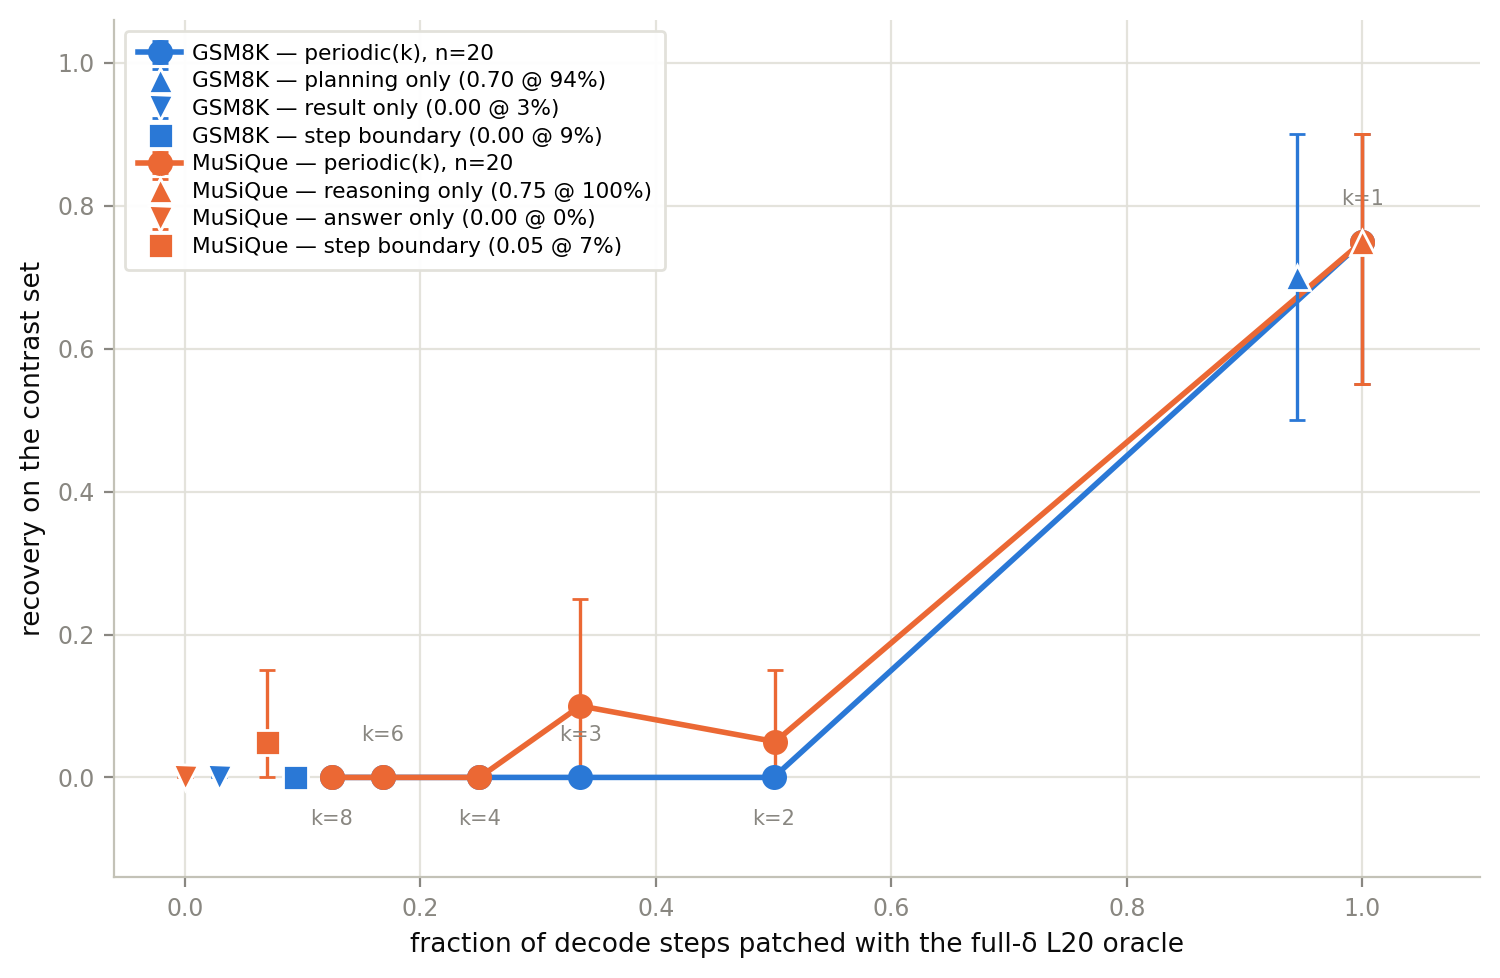
\includegraphics[width=0.72\linewidth]{figures/f1_temporal_density.png}
\caption{Temporal density of recovery. Periodic gates on the lockstep oracle: patching every step
recovers the budget; every-other-step collapses it; sparser gates are zero. Both procedures show
the same knee; the structural complement (patch everything except the answer span) equals the full
oracle. % TODO(F2..F6): five further figures — oracle layer sweeps (all three tasks), the ladder
% with intervals, the register-battery format/selection split, the criterion heatmap, the
% transplant/leak decomposition.
}
\label{fig:temporal}
\end{figure}

% ===================================================================================
\section{(G) A second procedure: the scaffold generalizes, the per-step work does not}
\label{sec:multihop}

One procedure cannot separate ``procedures do not install'' from ``arithmetic does not install,''
so we re-ran the apparatus end-to-end on MuSiQue open-book multi-hop QA \citep{trivedi2022musique}
(matched LoRA $0.000 \to 0.634$; 317 base-fail/donor-solve contrast problems).

\paragraph{The two structural axes replicate exactly.} \emph{Oracle:} the lockstep oracle at the
same layer recovers $+0.76$ (GSM8K $0.75$), all-layer control $+1.00$. \emph{Temporal density:}
patching every other step collapses recovery to $0.05$, every sparser periodic gate is
${\approx}0$, and the structural complement --- patch everything except the answer span --- equals
the full oracle, the same signature GSM8K gives. \emph{Plan vs.\ execute:} teacher-forcing the base
on the gold chain and lensing the gold token by its role, the base agrees with \textbf{execution}
tokens more than \textbf{planning} tokens ($+0.055$ \ci{+0.040}{+0.069}, bootstrapped over
problems), so the trajectory-control reading survives the task change --- and supplying the
trajectory makes the \emph{later}, nominally-composed hops \emph{easier} than the first
($+0.130$), which is what a trajectory deficit predicts and a per-step composition deficit does
not. What does \emph{not} carry over is the shape: where GSM8K's computed results sit $+0.133$
\ci{+0.096}{+0.173} above the chain average and crystallize with depth (lens rank $18 \to 7 \to 0$
over L20--24), multi-hop execution merely \emph{matches} the chain average ($+0.001$, interval
spanning 0) and no role crystallizes at all --- its hop answers are copies from the in-context
passages (the final restatement scores $0.933$ at lens rank 0 in every layer). The
trajectory-control deficit is general; the per-step work the base retains is task-specific, and
only on arithmetic is it computation rather than retrieval.

\paragraph{The ladder axis, matched at last --- and what the leak is.} The one place the two
procedures appeared to differ was the linear rung: multi-hop's ridge map leaks ($0.26$ at L20,
$0.45$ \ci{0.35}{0.56} at L24, a narrow $\alpha{=}1.0$ resonance) where GSM8K's was believed to
read ${\approx}0$. Measured at the same layers under the same protocol, GSM8K also leaks late ---
$0.09$--$0.12$ at L20/L24 (\S\ref{sec:ladder}) --- so the divergence survives only as
\emph{degree}, not kind.
% TODO(refit): MuSiQue's 0.45 is still a CoT-window fit; the all-positions re-fit is queued. Until
% it lands, state the cross-task ratio as unmatched-fit-windows or update it from the new artifact.
Two further measurements say what the leak is made of. \textbf{It is task-agnostic:} maps fit on
\emph{multi-hop} $\delta$s and applied to GSM8K deliver 75--100\% of the native leak (L24 $0.09$
\ci{0.05}{0.16} vs.\ native $0.12$; L28 $0.13$, equal to native exactly), so the task-fitted
component transports ${\leq}0.03$ --- the leak is a late-stack \emph{register push}, not
transported procedure. \textbf{And better fit means less transport:} at the live layer the MLP head
fits $\delta$ better than ridge ($\cos 0.815$ vs.\ $0.656$, $R^2$ $0.675$ vs.\ $0.354$) and
transports \emph{nothing} ($0.00$ \ci{0}{0.04} vs.\ ridge $0.10$ \ci{0.05}{0.18}, disjoint
intervals) --- the transportable component is the \emph{unconditional} one, which the better
estimator correctly attributes to the conditional structure it cannot transport.

% ===================================================================================
\section{(R) The register battery: the other half of the boundary, measured}
\label{sec:battery}

The claim so far is two-sided but the battery was one-sided: both procedures have an oracle sweep,
a temporal knee, and a null ladder; the register side rested on refusal alone. We therefore pointed
the \emph{unmodified} procedure drivers at a register donor: a commonsense LoRA (r32, same recipe
as \S\ref{sec:routes}) whose target is the ${\sim}7$-token template ``\texttt{the correct answer is
answerX}'' on ARC-Challenge, with a 338-problem contrast set (base $0.000$ / donor $0.676$).
ARC-Challenge is 4-way, so a garbled intervention cannot pass by coin-flip: the measured floors are
$0.25$ (chance) and $0.288$ (majority class).

\paragraph{The oracle itself separates register from procedure.} Under the same driver and the same
earliest-plateau rule, all three tasks select $L^{*}{=}20$ --- but the curves differ in exactly the
way the two-kinds view predicts (Table~\ref{tab:oracle}). The register's onset is earlier and far
sharper ($0.830$ at L16, where MuSiQue reads $0.020$), and its plateau is essentially total
($0.990$ against $0.75/0.76$). The onset comparison is within-task-across-layer and thus immune to
generation-length effects; the ceiling comparison is not (the register's target is ${\sim}7$ tokens
against 256--512-token chains), and we flag it accordingly.

\begin{table}[t]
\centering
\caption{Single-layer lockstep oracle recovery by task ($n{=}100$ contrast problems each). Layers
28/31 are degenerate (block-output overwrite) and excluded from $L^*$ selection.
% TODO(F2): fill the GSM8K column from the per-layer sweep now running
% (lockstep_gsm8k_single_sweep.json); only the L20 cell is currently doubly-sourced.
}
\label{tab:oracle}
\small
\begin{tabular}{lccc}
\toprule
layer & commonsense (register) & MuSiQue & GSM8K \\
\midrule
12 & 0.050 & 0.020 & \emph{TODO(F2)} \\
16 & \textbf{0.830} & 0.020 & \emph{TODO(F2)} \\
20 & \textbf{0.990} & 0.760 & 0.750 \\
24 & 0.990 & 0.780 & \emph{TODO(F2)} \\
\bottomrule
\end{tabular}
\end{table}

\paragraph{The fitted map installs the register --- completely, and at one layer.} Fit on all
positions (the fit window must match the application window; fitting on generated positions only
and applying everywhere destroys the model --- a failure mode we hit, diagnosed from decoded
generations, and now test for), the ridge map's \emph{format compliance} at $\alpha{=}0.75$ on the
500-problem scan is: L16 $0.140$, \textbf{L20 $0.972$}, L24 $0.998$ (base $0.004$, donor $1.000$).
Set beside the same instrument on the procedures --- GSM8K $0.03/0.12$, MuSiQue $0.26/0.45$ at
L20/L24 --- this is the boundary on one axis: \emph{a register transports through a fitted
pointwise map at a single layer; a procedure does not.}

\paragraph{It installs the register and destroys the selection the base already had.} Under the
map, accuracy equals the base rate of a constant policy --- $0.200$ with gold-\texttt{answer1} at
$8/40$, replicated at $0.267$ with $16/60$ --- and there is no $\alpha$ that installs and selects:
$\alpha{=}1.24$, which magnitude-matches the donor's shift, collapses format itself to $0.083$.
Meanwhile the contrast set turns out to be ${\sim}$two-thirds \emph{format}: base scores $0.630$
with a 4-shot prompt, and a scrambled-label control also scores exactly $0.630$, so the exemplars
supply format and nothing else. Three interventions, one table: the CAA-style fixed vector installs
neither format nor selection ($0.000$); the fitted map installs format and \emph{destroys}
selection ($0.200$, a constant policy); the 4-shot prompt installs the same format and leaves
base's own selection intact ($0.630$). The weight-route register install costs something the
prompt-route install does not. Consequently the oracle's $0.990$ must not be described as
recovering a capability base lacks --- it is substantially format installation, and we say so.

\paragraph{No vector estimated once installs anything.} A per-problem trajectory-mean vector
through an additive hook: $0.000$. The same vector through the oracle's own delivery path:
$0.000$. A pooled vector over 100 disjoint problems, at $\alpha \in \{0.5, 1, 1.5, 2\}$: $0.000$.
On the \emph{temporal} axis, then, the register behaves like the procedures --- a
deployable-in-principle fixed vector installs nothing --- and the boundary lives in the oracle's
onset/ceiling and in the fitted map, not in ``the register is one direction.'' It is not: the
centred held-out $R^2$ of the register's map is $0.921$ (constant baseline $0.106$), the required
shift rotates substantially within a 7-token generation, and a matched-norm \emph{coherent} random
direction --- injected through the same plumbing that installs the register when given the mean-\,$\delta$
direction --- reads $0.000$ with base-like generations. A per-step statistic that collapses the
shift across \emph{positions} but keeps a live donor in the loop retains $0.860$ of the oracle;
collapsing across \emph{time} is what kills it. Direction is everything; magnitude alone is
nothing.

% ===================================================================================
\section{A measured criterion for installability}
\label{sec:criterion}

Table~\ref{tab:criterion} assembles the coordinates this paper measured. We propose them as a
falsifiable criterion: a behavior installs through a pointwise conditional map iff its required
shift is (i) transportable at a single layer (map arm), (ii) recovered by the oracle with early,
sharp onset, and (iii) not time-dense at the trajectory level. Cells we did not measure are marked
--- a criterion is only as good as its unmeasured cells are visible.

\begin{table}[t]
\centering
\caption{The criterion table. ``n.m.'' = not measured (stated, not estimated). Ridge cells for the
procedures are lower bounds (\S\ref{sec:ladder}).
% TODO(F2): GSM8K oracle onset cell. TODO(refit): MuSiQue map cell under matched fit window.
}
\label{tab:criterion}
\small
\setlength{\tabcolsep}{4pt}
\begin{tabular}{lcccc}
\toprule
 & refusal & commonsense register & GSM8K & MuSiQue \\
\midrule
map transport (single layer) & 0.62 (Pareto) & 0.972 (format) & 0.09--0.12 & 0.26--0.45 \\
oracle onset / plateau & n.m.\ / n.m. & L16 0.830 / 0.990 & \emph{TODO(F2)} / 0.75 & L16 0.020 / 0.76 \\
fixed vector (time-collapsed) & 0.00 & 0.000 & 0.00 & n.m. \\
centred held-out $R^2$ of $\delta$ & ${\approx}1.0$ & 0.921 & 0.653 & n.m. \\
temporal density (periodic-2 gate) & n.m. & n.m.\ (7-token target) & ${\to}0.00$ & 0.05 \\
$\delta$-rank / variance band & n.m. & n.m.\ (cut) & 80\% band needed & n.m. \\
\bottomrule
\end{tabular}
\end{table}

Two readings the table supports, and one it does not. It supports: registers sit in the
top-left corner (high map transport, early sharp oracle onset) and procedures in the bottom-right
(map transport at leak level only, late onset, time- and variance-dense); and the coordinate that
does \emph{not} separate the two sides is the constancy of $\delta$ ($R^2_{\mathrm{const}}$
$0.096$ vs.\ $0.106$ at L20) --- the discriminator is the \emph{centred} $R^2$, i.e.\ how
predictable the \emph{conditional} part of the shift is. It does not support: any claim about
behaviors outside this table. Sycophancy, sentiment, induction --- the held-out behaviors that
would turn this from a summary into a criterion --- are future work, and the table's own empty
cells show what measuring one costs.

% ===================================================================================
\section{(X) Cross-model: the disposition carries; better aim transports worse}
\label{sec:crossmodel}

Transplanting a trained LoReFT edit from a donor (Llama-2-7B base) to a recipient (Llama-2-7B-chat)
through a per-layer orthogonal-Procrustes bridge transfers the \emph{disposition} off-policy (BoolQ
boolean-commitment $32 \to 53/64$, lenient $0.33 \to 0.58$) but not the trained output template or
answer correctness (exact-match ${\approx}0$). On-policy refit is \emph{worse}; and a ridge-fit
\textbf{affine} bridge with 12--45$\times$ better held-out geometry transports the edit \emph{worse
still} ($8/64$), because the LoReFT delta lives off the data manifold
($\lVert\delta\rVert > \lVert h\rVert$) and regression shrinks weakly-represented directions ---
precisely the ones that must be preserved \citep{oozeer2025transfer}. Strength beats aim: full-norm
deltas through a crude isometry move behavior; well-aimed deltas at half norm do nothing. The
geometric ``wall'' was real but behaviorally irrelevant --- consistent with \S\ref{sec:multihop}'s
finding that the better-fitting estimator transports less.

% ===================================================================================
\section{Synthesis and limitations}
\label{sec:synthesis}

One axis organizes the results. A \textbf{register} --- refusal tone, an answer format --- is an
on-manifold, input-conditional but \emph{pointwise-transportable} function of the activation: a
single-layer closed-form map installs it (0.62 Pareto; 0.972 format), and even a crude cross-model
rotation carries its coarse disposition. A \textbf{procedure} is a distributed, time-dense,
variance-dense \emph{trajectory state}: invisible to every pointwise estimator we fit (the better
the fit, the less transports), recoverable only by supplying the donor's near-full state at almost
every step. Finetuning and steering are the same map family and inherit the same boundary: they
relocate \emph{where a disposition points}, not \emph{how a computation unfolds}. And the boundary
is visible from both sides of the same instrument: the register's oracle onset is early and sharp
where the procedures' is late; the register's map installs the surface completely --- at the price
of the selection the base already had --- where the procedures' map carries only a task-agnostic
register push.

\paragraph{Limitations.} (1)~Everything here is Llama-2-7B; the apparatus requires only a Llama
layer layout and a trained donor, so cross-model replication is mechanical, but it has not been
done. (2)~$n{=}2$ procedures and $n{=}2$ registers; the criterion table names what a third of each
costs. (3)~The register's oracle \emph{ceiling} comparison carries a generation-length confound
(7-token vs.\ 256--512-token targets); the onset claim does not, and we lead with onset.
(4)~The register-side geometry (map-vs-donor cosine $0.788$; few-shot route ${\sim}70^{\circ}$
away) awaits a length-matched control before ``format direction'' language is licensed, and we do
not use it. (5)~Two criterion cells are lower bounds ($\alpha$ peaks not located) and several are
unmeasured; they are marked in the table rather than extrapolated.

\bibliographystyle{plainnat}
\bibliography{refs}

\end{document}
